\documentclass{beamer}
\usepackage[utf8]{inputenc}

\usetheme{Madrid}
\usecolortheme{default}
\usepackage{amsmath,amssymb,amsfonts,amsthm}
\usepackage{txfonts}
\usepackage{tkz-euclide}
\usepackage{listings}
\usepackage{adjustbox}
\usepackage{array}
\usepackage{tabularx}
\usepackage{gvv}
\usepackage{lmodern}
\usepackage{circuitikz}
\usepackage{tikz}
\usepackage{graphicx}
\usepackage{amsmath}

\setbeamertemplate{page number in head/foot}[totalframenumber]

\usepackage{tcolorbox}
\tcbuselibrary{minted,breakable,xparse,skins}



\definecolor{bg}{gray}{0.95}
\DeclareTCBListing{mintedbox}{O{}m!O{}}{%
  breakable=true,
  listing engine=minted,
  listing only,
  minted language=#2,
  minted style=default,
  minted options={%
    linenos,
    gobble=0,
    breaklines=true,
    breakafter=,,
    fontsize=\small,
    numbersep=8pt,
    #1},
  boxsep=0pt,
  left skip=0pt,
  right skip=0pt,
  left=25pt,
  right=0pt,
  top=3pt,
  bottom=3pt,
  arc=5pt,
  leftrule=0pt,
  rightrule=0pt,
  bottomrule=2pt,
  toprule=2pt,
  colback=bg,
  colframe=orange!70,
  enhanced,
  overlay={%
    \begin{tcbclipinterior}
    \fill[orange!20!white] (frame.south west) rectangle ([xshift=20pt]frame.north west);
    \end{tcbclipinterior}},
  #3,
}
\lstset{
    language=C,
    basicstyle=\ttfamily\small,
    keywordstyle=\color{blue},
    stringstyle=\color{orange},
    commentstyle=\color{green!60!black},
    numbers=left,
    numberstyle=\tiny\color{gray},
    breaklines=true,
    showstringspaces=false,
}


\title 
{4.8.19}



\author 
{Pratik R-AI25BTECH11023}



\begin{document}


\frame{\titlepage}
%------------------------------------
\begin{frame}{Question}
If the distance of the point $(1,1,1)$ from the plane $x-y+z+ \lambda = 0$ is$\frac{5}{\sqrt{3}}$, find the value(s) of $\lambda$.
\end{frame}
\begin{frame}{Solution} 
Equation of plane is given by
\begin{align}
	\vec{n}^\top \vec{x} = -\lambda;
\end{align}
	where $\vec{n}^\top = \myvec{1&-1&1}$. 
\end{frame}
\begin{frame}{Solution}
	Let the distance of point \vec{P}(1,1,1) from the plane is d.
\begin{align}
	d = \dfrac{||\vec{n}^\top \vec{P} + \lambda||}{||\vec{n}||}
\end{align}
then value of $\lambda $ is given by
\begin{align}
	\lambda = + d||\vec{n}||-\vec{n}^\top \vec{\vec{P}} \text{ or} \\
	\lambda = - d||\vec{n}||-\vec{n}^\top \vec{\vec{P}}
\end{align}
Solving these Equations we get
\begin{align}
   \implies \lambda &= +4 \\
    &=-6
\end{align}
\end{frame}
\begin{frame}{plot}
\centering
    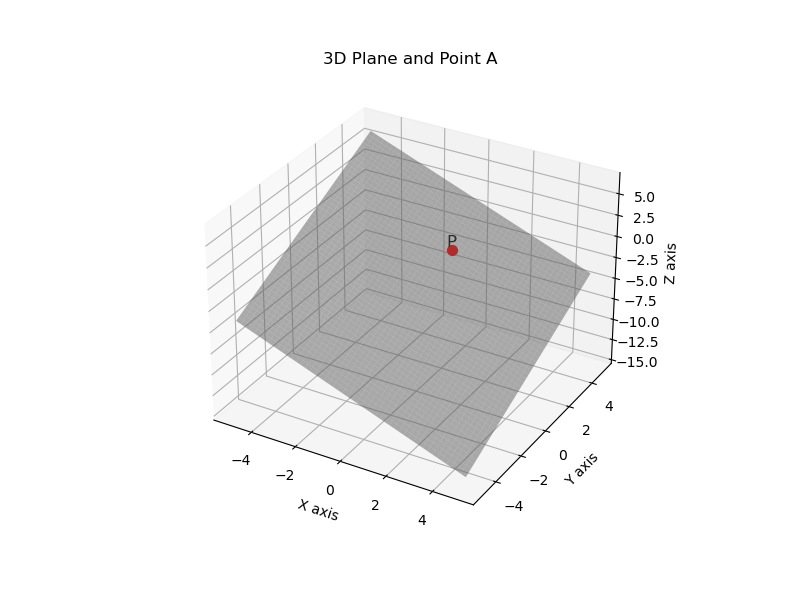
\includegraphics[width=\columnwidth, height=0.8\textheight, keepaspectratio]{../figs/fig1.png}     
\end{frame}
\begin{frame}{plot}
\centering
    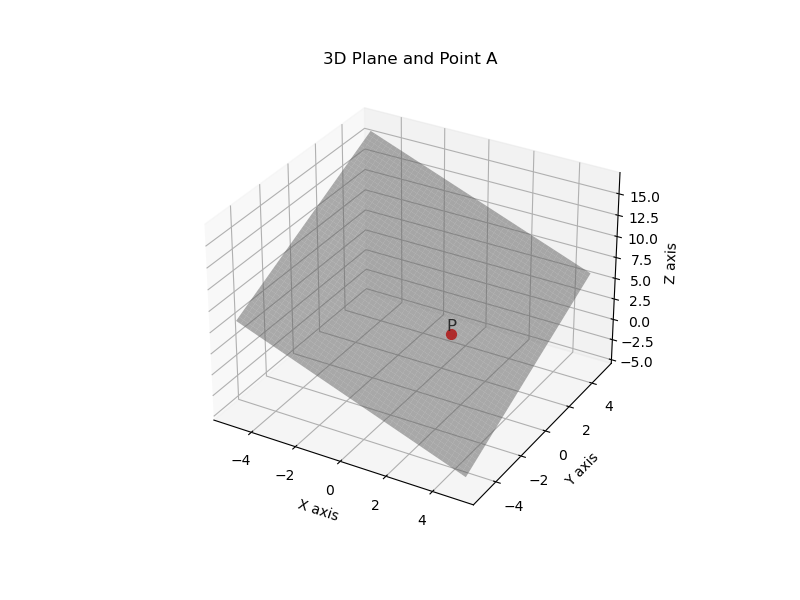
\includegraphics[width=\columnwidth, height=0.8\textheight, keepaspectratio]{../figs/fig2.png}     
\end{frame}

\end{document}
